\documentclass[12pt]{article}
\usepackage{geometry} % For setting page margins
\usepackage{hyperref} % For hyperlinks
\usepackage{listings} % For code listings
\usepackage{amsmath, amssymb, amsthm} % For math symbols, theorems
\usepackage{graphicx} % For including images
\usepackage{fancyhdr} % For headers and footers
\usepackage{xcolor} % For color definitions
\usepackage{titling}
\usepackage{graphicx}
\usepackage{float}
\usepackage{bm}
\usepackage{mdframed}
\usepackage{etoolbox}


% Prevent widow and orphan lines
\widowpenalty=10000
\clubpenalty=10000

% Avoid extra page breaks after sections
\makeatletter
\patchcmd{\@startsection}
{\@afterindenttrue}
{\@afterindentfalse}
{}{}
\makeatother

% Use ragged bottom to reduce vertical stretching
\raggedbottom

% subsubsubsection = paragraph
\setcounter{tocdepth}{4}
\setcounter{secnumdepth}{4}

% Define gray color
\definecolor{gray}{rgb}{0.5,0.5,0.5}

% Adjust spacing in itemize environment globally
\usepackage{enumitem}
\setlist[itemize]{itemsep=0.2em, parsep=0em, topsep=0em}

% Page layout
\geometry{a4paper, margin=1in}
\setlength{\parskip}{1em} % Add space between paragraphs
\setlength{\parindent}{0pt} % No indentation for new paragraphs

% Header and Footer
\pagestyle{fancy}
\fancyhf{}
\fancyhead[L]{User's Guide: Dynamic Optimization}
\fancyfoot[C]{\thepage}

% Colors for code
\definecolor{commentgreen}{rgb}{0,0.6,0}
\definecolor{keywordblue}{rgb}{0,0,0.9}
\definecolor{stringred}{rgb}{0.6,0,0}

% Python code listing
\lstset{
	language=Python,
	basicstyle=\ttfamily\small,
	keywordstyle=\color{keywordblue},
	stringstyle=\color{stringred},
	commentstyle=\color{commentgreen},
	showstringspaces=false,
	columns=flexible,
	breaklines=true,
	breakatwhitespace=true,
	numbers=left,
	numberstyle=\tiny\color{gray},
	frame=single,
	captionpos=b,
	xleftmargin=2em,
	xrightmargin=2em,
	aboveskip=1em,
}

\newtheorem{definition}{Definition}
\newcommand{\dd}{\mathrm{d}}
\newcommand{\coloredtextbf}[1]{\textbf{\textcolor{blue}{#1}}}
% maybe use in the future or different: good, neutral, evil :)
\renewcommand{\v}{\bm}
\date{\today}

\begin{document}

\begin{titlepage}
	\centering

	\vspace*{2cm}

	{\Huge\bfseries User's Guide:}\\[1em]

	{\Huge\bfseries Dynamic Optimization Framework}\\[0.5em]
	\textcolor{gray}{\large A Python-based Environment for Solving
		Dynamic Models}\\[1em]

	\vspace{2cm}

	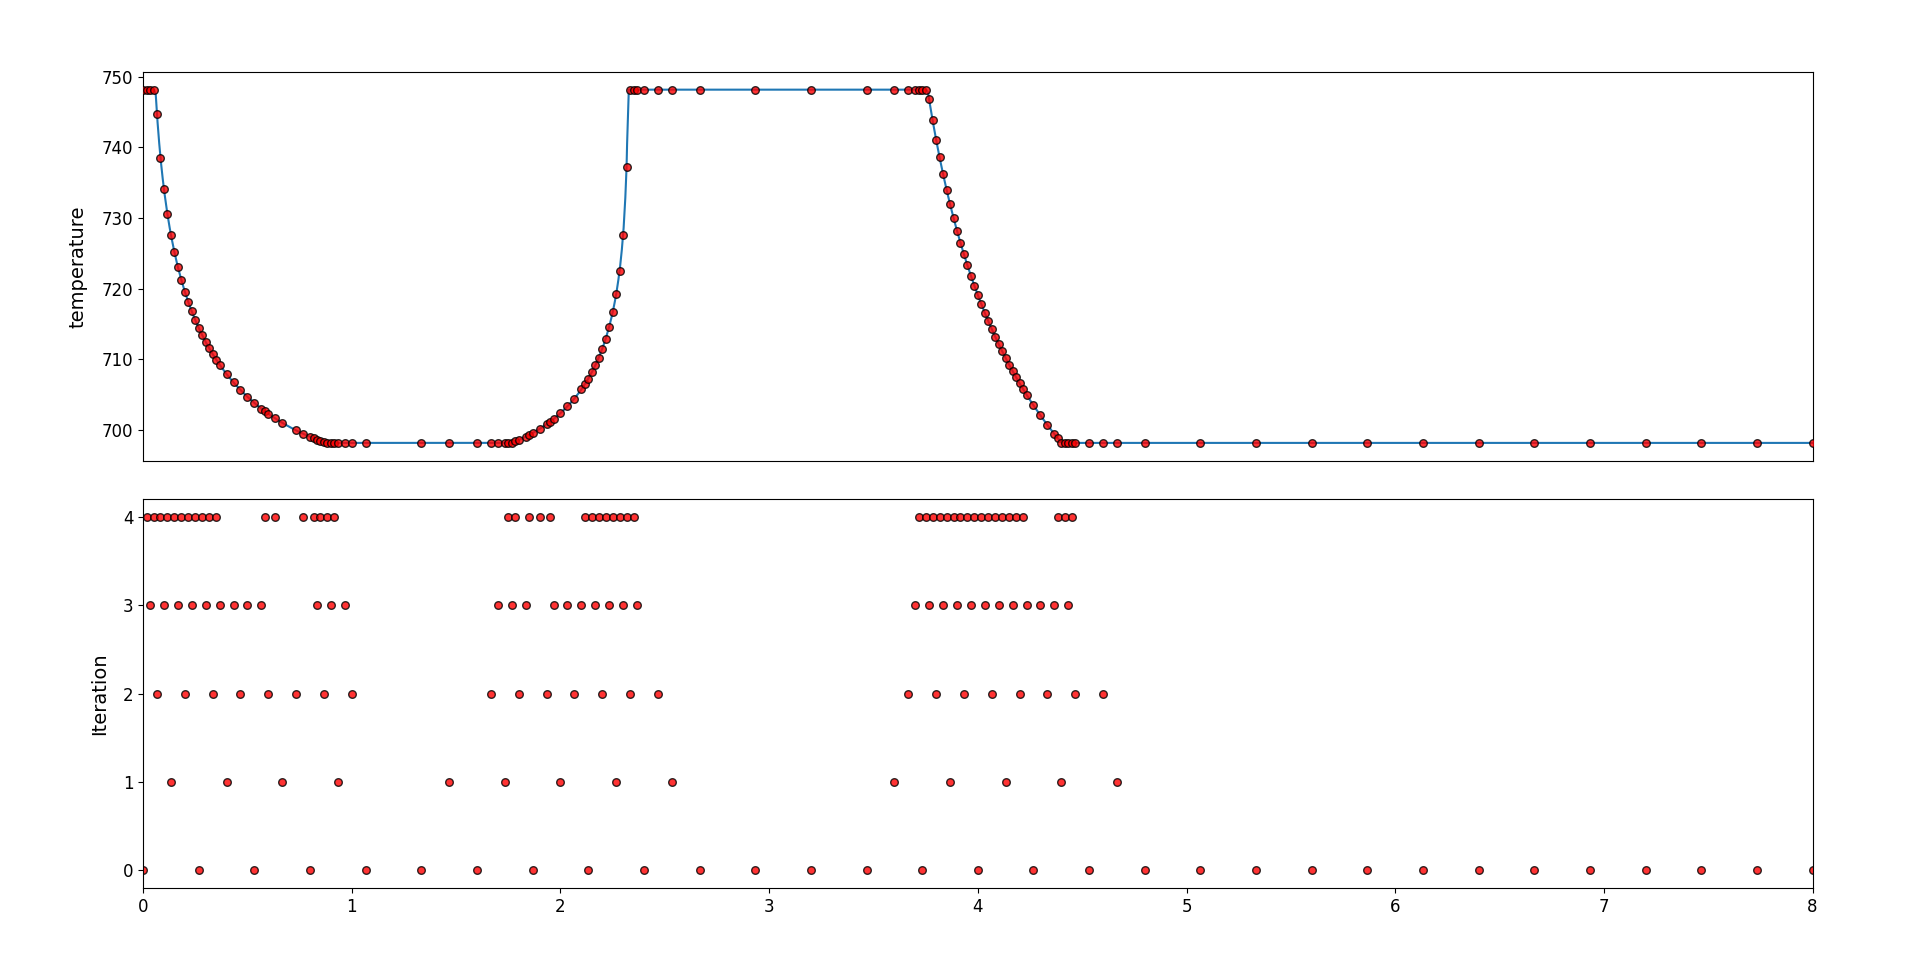
\includegraphics[width=1\textwidth]{images/refinement.png}\par\vspace{1cm}
	\vspace{2cm}

	{\large \textit{Author:}}\\[0.5em]
	{\large Linus Langenkamp}

	\vfill

	{\large \today}

	\vspace*{1cm}
\end{titlepage}

\newpage
\tableofcontents
\newpage

\section{Introduction}

Dynamic optimization is a branch of mathematical optimization that
deals with systems evolving over time. It aims to find the optimal trajectory
of a system's state variables by adjusting control inputs while respecting
constraints over a defined time horizon. Such problems arise in various fields,
including control theory, economics, engineering or industrial biochemistry.

This guide presents a high level Python modeling environment for
solving dynamic optimization problems using local collocation methods and
adaptive mesh refinement techniques. The following sections provide
step-by-step instructions on setting up, modeling and optimizing dynamic models
along with analyzing the optimal solution.

\subsection{How Does the Framework Solve Dynamic Models?}
\label{c:collocation}

\section{Installation}
Clone the repository from GitHub:

\begin{lstlisting}[language=bash]
git clone https://github.com/linuslangenkamp/DynamicOptimization.git
	\end{lstlisting}

\subsection{Requirements}
Ensure that the following dependencies are installed:
\begin{itemize}

	\item[$\bullet$] Optimizer

		\begin{itemize}
			\item[$\bullet$] IPOPT
		\end{itemize}

	\item[$\bullet$] Linear Solver (one of the below)

		\begin{itemize}
			\item[$\bullet$] MUMPS
			\item[$\bullet$] HSL solvers, such as MA27, MA57, MA86,
				\ldots
		\end{itemize}

	\item[$\bullet$] Frontend Python Packages

		\begin{itemize}
			\item[$\bullet$] SymEngine
			\item[$\bullet$] NumPy
			\item[$\bullet$] SciPy
			\item[$\bullet$] pandas
			\item[$\bullet$] Matplotlib
		\end{itemize}
\end{itemize}

\section{Getting Started}
This section will show how to set up and solve a simple dynamic
optimization problem with the proposed framework.

\subsection{Basic Example}
Here is a minimal working example for a bang-bang control problem,
adapted from the OpenModelica User's
Guide\footnote{\url{https://openmodelica.org/doc/OpenModelicaUsersGuide/latest/optimization.html}}:

\begin{lstlisting}
from optimization import *

model = Model("bangBang")

# states x1(t), x2(t) with x1(0) = x2(0) = 0
x1 = model.addState(start=0, symbol="obj") 
x2 = model.addState(start=0, symbol="obj'")

# control: u(t) with |u(t)| <= 10
u = model.addControl(lb=-10, ub=10, symbol="control") 

# dynamic: x1''(t) = u(t)
model.addDynamic(x1, x2) # x1'(t) = x2(t)
model.addDynamic(x2, u)  # x2'(t) = u(t)

# algebraic constraints
model.addPath(x2 * u, lb=-30, ub=30) # -30 <= x2(t) * u(t) <= 30
model.addFinal(x2, eq=0) # x2(tf) = 0

# objective = x1(tf) -> max
model.addMayer(x1, Objective.MAXIMIZE) 

# generate the C++ code
model.generate() 

# tf=0.5s, 150 intervals, using RadauIIA 3 step order 5 scheme
model.optimize(tf=0.5, steps=150, rksteps=3)

model.plot()
	\end{lstlisting}

\subsection{Explanation}
Example procedure:
\begin{itemize}
	\item Import the package and create a \texttt{Model} object
	      with a given name
	\item Add the states with given starting values (and optionally
	      assign a symbol)
	\item Add the control with lower and upper bounds (and
	      optionally assign a symbol)
	\item Define the dynamic, path, final constraints
	\item Add a objective
	\item Generate the C++ code
	\item Optimize for a given final time, number of steps and
	      collocation nodes
	\item Plot the model
\end{itemize}

\subsection{Solution}

\begin{figure}[H]
	\centering
	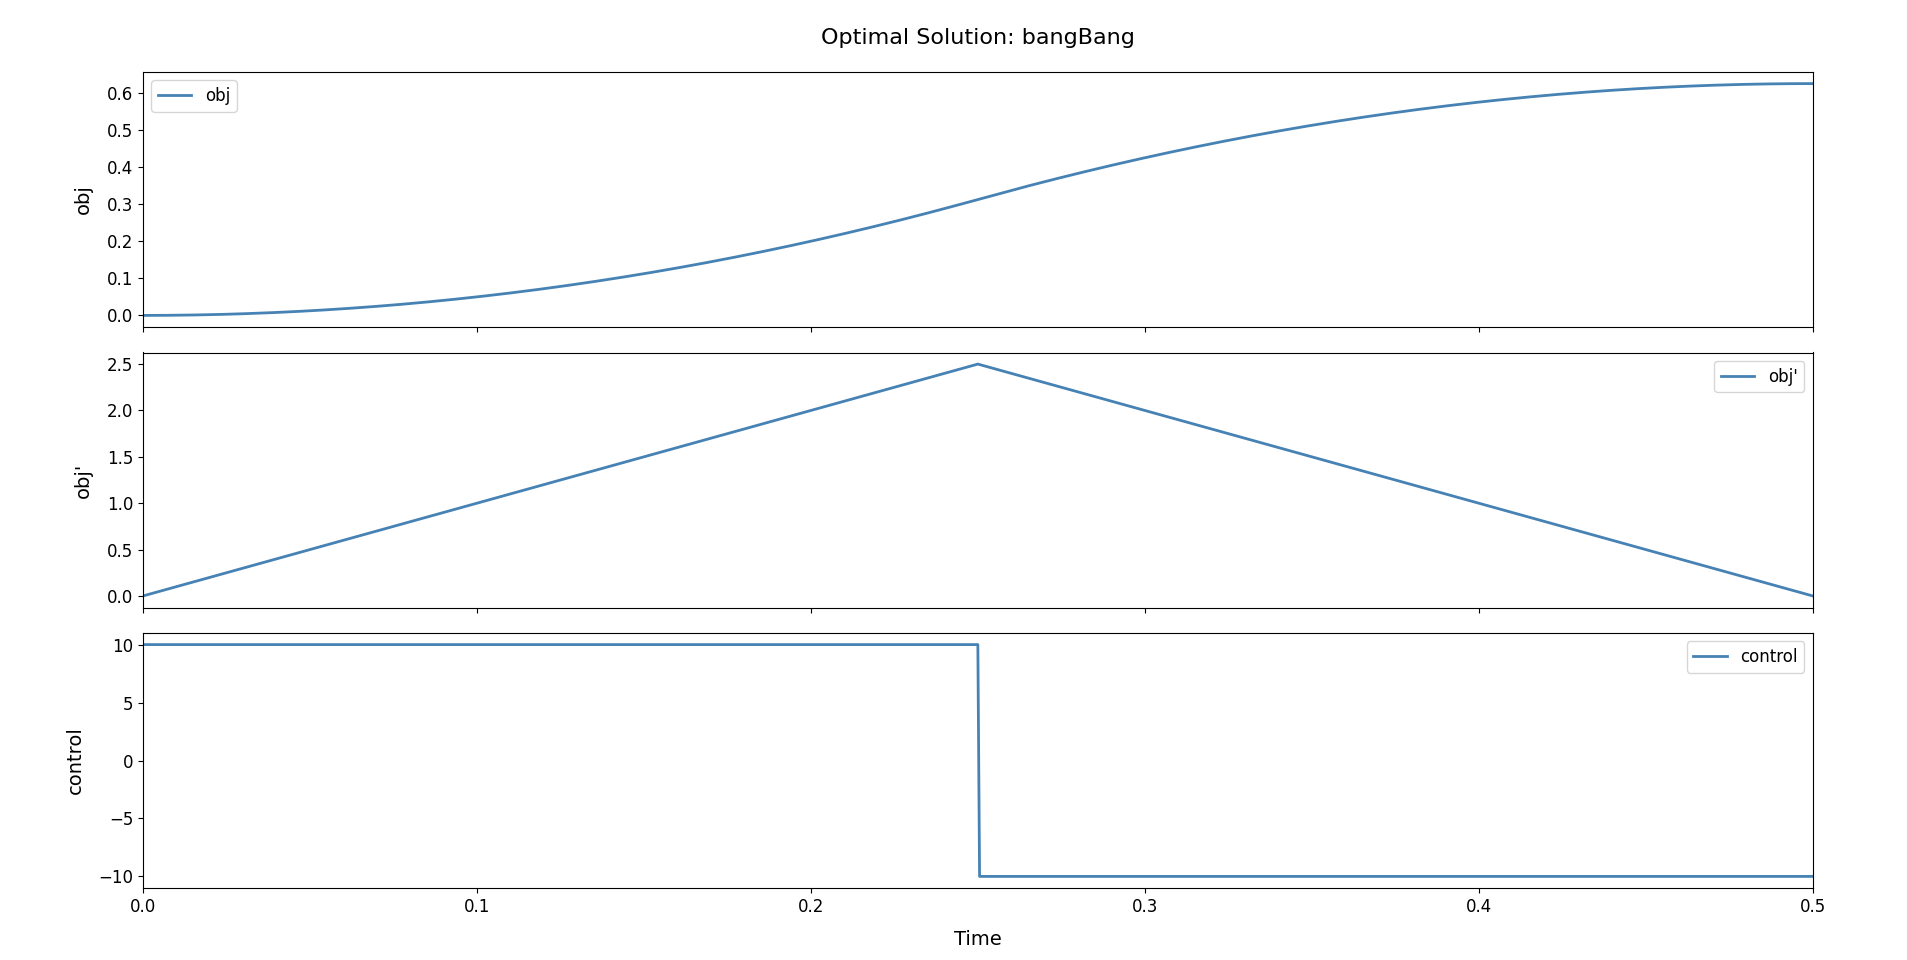
\includegraphics[width=\textwidth]{images/bangBang.png}
	\caption{Optimal bang-bang solution provided by the framework}
	\label{fig:bangBang}
\end{figure}

\section{Mathematical Problem Formulation}
\label{c:GDOP}
\begin{definition}[General Dynamic Optimization Problem]
	\begin{align*}
		\min_{\v{u}(t), \v{p}} ~ & M(\v{x}(t_f), \v{u}(t_f),
		\v{p}, t_f) + \int_{t_0}^{t_f} L(\v{x}(t), \v{u}(t), \v{p}, t)
		\, \mathrm{d}t
		\\
		\text{s.t.}              &
		\\
		\dot{\v{x}}(t)           & = \v{f}(\v{x}(t), \v{u}(t), \v{p},
		t)\
		\forall t \in [t_0, t_f]
		\\
		\v{x}(t_0)               & = \v{x}_0
		\\
		\v{g}^{L}                & \leq \v{g}(\v{x}(t), \v{u}(t),
		\v{p}, t)
		\leq \v{g}^{U}\ \forall t \in [t_0, t_f]
		\\
		\v{r}^{L}                & \leq \v{r}(\v{x}(t_f), \v{u}(t_f),
		\v{p},
		t_f) \leq \v{r}^{U}
		\\
		\v{a}^{L}                & \leq \v{a}(\v{p}) \leq \v{a}^{U}
	\end{align*}
\end{definition}

\subsection{Variables}

\subsection{Constraints}

\subsection{Objective}
Variables:
\\
$u(t)$ is the time-dependent control, $p$ is a set of static
parameters, $t_f$ is the final time.
\\
Objective:
\\
With the Mayer term $M(\cdot)$ evaluating the final state, and the
Lagrange term $L(\cdot)$ aggregating desired combinations of states.
\\
Constraints:
\\
With $\dot{x} = f(\cdot)$ and $x(t_0) = x_0$ as the initial value
problem for the states, $g^L \leq g(\cdot) \leq g^U$ as the path constraints
for the states and control over the entire time horizon, $h^L_k \leq h_k(\cdot)
	\leq h^U_k$ as the path constraints for subsets of the time horizon,
$r^L \leq
	r(\cdot) \leq r^U$ as the final constraints for the states and control,
and
$a^L \leq a(p) \leq a^U$ as the algebraic constraints for the parameters.

\section{Modeling}

The first step is to create a new Python file and to import the
\texttt{optimization} package.
\begin{lstlisting}
from optimization import *
	\end{lstlisting}

Additionally a \texttt{Model} object has to be created. This
\texttt{Model} is the basis for any modeling and has to have an associated
model name.
\begin{lstlisting}
model = Model("Model Name")
	\end{lstlisting}

The variables, constraints and objectives will be added to this
\texttt{Model} object.

\subsection{Variables}

\subsubsection{States}

States are time-dependent functions, that will be calculated in the
solving process. The value of the state is completely determined by a starting
value and an ordinary differential equation.

\begin{mdframed}[backgroundcolor=gray!10, roundcorner=10pt, linewidth=1pt]

	Adding a state to a \texttt{Model} object.

	\begin{lstlisting}
x = model.addState(start, symbol=None, lb=-float("inf"), ub=float("inf"), nominal=None)
	\end{lstlisting}

	\textbf{Parameters:}
	\begin{itemize}
		\item \texttt{float start}: The initial value of the state
		      variable.
		\item \texttt{str symbol} \emph{(optional)}: A symbolic
		      representation of the state. The state will be
		      represented by this symbol in
		      further analysis.
		\item \texttt{float lb} \emph{(optional)}: Lower bound for the
		      state variable.
		\item \texttt{float ub} \emph{(optional)}: Upper bound for the
		      state variable.
		\item \texttt{float nominal} \emph{(optional)}: A nominal value
		      for scaling.
	\end{itemize}

	\textbf{Returns:}
	\texttt{Symbol variable}: The symbolic representation of the state
	variable, which can be used in constraints.

	\textbf{Aliases:} \texttt{model.addX}
\end{mdframed}

\subsubsection{Inputs}

Input are time-dependent functions, that will be calculated in the
solving process and are not differentiated in the model.

\begin{mdframed}[backgroundcolor=gray!10, roundcorner=10pt, linewidth=1pt]

	Adding a input variable $u(t)$, that changes over time, to a
	\texttt{Model} object.

	\begin{lstlisting}
u = model.addInput(symbol=None, lb=-float("inf"), ub=float("inf"), guess=0, nominal=None)
	\end{lstlisting}
	\label{addInput}
	\textbf{Parameters:}
	\begin{itemize}
		\item \texttt{str symbol} \emph{(optional)}: A symbolic
		      representation of the input. The input will be
		      represented by this symbol in
		      further analysis.
		\item \texttt{float lb} \emph{(optional)}: Lower bound for the
		      input variable.
		\item \texttt{float ub} \emph{(optional)}: Upper bound for the
		      input variable.
		\item \texttt{Expression guess} \emph{(optional)}: An initial
		      guess for the input. Further explanation in
		      \ref{p:cguesses}.
		\item \texttt{float nominal} \emph{(optional)}: A nominal value
		      for scaling.
	\end{itemize}

	\textbf{Returns:}
	\texttt{Symbol variable}: The symbolic representation of the input,
	which can be used in constraints.

	\textbf{Aliases:}  \texttt{model.addU}, \texttt{model.addControl},
	\texttt{model.addContinuous}
\end{mdframed}

\paragraph{Input Guesses}
\label{p:cguesses}
The guess parameter in \texttt{model.addInput} (\ref{addInput}) can be
any \texttt{Expression} that contains the global time or final time symbols
\ref{c:globaltime}, but can also be a regular constant \texttt{float} or
\texttt{int}. This guess trajectory is only used if the
\texttt{"initVars"} flag \ref{flag:initVars} is chosen to be
\texttt{InitVars.SOLVE} \ref{enum:initVars}. This trajectory will be used to
solve the dynamic and provide an initial, feasible guess for the state
variables. Note that any valid SymEngine \texttt{Expression} can be provided as
a guess, although there are several standard functions to provide better
initial guesses for the control.

\begin{mdframed}[backgroundcolor=gray!10, roundcorner=10pt, linewidth=1pt]

	Providing a constant control guess trajectory.

	\begin{lstlisting}
guessConstant(const)
	\end{lstlisting}

	\textbf{Parameters:}
	\begin{itemize}
		\item \texttt{float const}: Constant value for the control
		      guess, i.e. $u(t) \equiv const ~ \forall t \in [0, t_f]$.
	\end{itemize}

	\textbf{Remarks:} It's also possible to just write \texttt{guess=const}
	in the \texttt{model.addInput} arguments.
\end{mdframed}

\begin{mdframed}[backgroundcolor=gray!10, roundcorner=10pt, linewidth=1pt]

	Providing a linear control guess trajectory. The provided values will
	be interpolated accordingly.

	\begin{lstlisting}
guessLinear(u0, uf)
	\end{lstlisting}

	\textbf{Parameters:}
	\begin{itemize}
		\item \texttt{float u0}: Value for the control guess at $t=0$,
		      i.e. $u(0)$.
		\item \texttt{float uf}: Value for the control guess at
		      $t=t_f$, i.e. $u(t_f)$.
	\end{itemize}

\end{mdframed}

\begin{mdframed}[backgroundcolor=gray!10, roundcorner=10pt, linewidth=1pt]

	Providing a quadratic control guess trajectory. The provided values
	will be interpolated accordingly.

	\begin{lstlisting}
guessQuadratic(u0, um, uf)
	\end{lstlisting}

	\textbf{Parameters:}
	\begin{itemize}
		\item \texttt{float u0}: Value for the control guess at $t=0$,
		      i.e. $u(0)$.
		\item \texttt{float um}: Value for the control guess at
		      $t=\frac{t_f}{2}$, i.e. $u(\frac{t_f}{2})$.
		\item \texttt{float uf}: Value for the control guess at
		      $t=t_f$, i.e. $u(t_f)$.
	\end{itemize}

\end{mdframed}

\begin{mdframed}[backgroundcolor=gray!10, roundcorner=10pt, linewidth=1pt]

	Providing a exponential control guess trajectory. The provided values
	will be interpolated accordingly.

	\begin{lstlisting}
guessExponential(u0, uf)
	\end{lstlisting}

	\textbf{Parameters:}
	\begin{itemize}
		\item \texttt{float u0}: Value for the control guess at $t=0$,
		      i.e. $u(0)$.
		\item \texttt{float uf}: Value for the control guess at
		      $t=t_f$, i.e. $u(t_f)$.
	\end{itemize}

\end{mdframed}

\begin{mdframed}[backgroundcolor=gray!10, roundcorner=10pt, linewidth=1pt]

	Providing a piecewise defined control guess trajectory.

	\begin{lstlisting}
guessPiecewise(*args)
	\end{lstlisting}

	\textbf{Parameters:}
	\begin{itemize}
		\item \texttt{*(Expression, Condition) *args}: Arbitrary number
		      of tuples with an Expression as the first and the
		      corresponding interval its
		      defined on as second argument.
	\end{itemize}

	\textbf{Example:} \texttt{guessPiecewise((0.6, t <= 0.5), (2 + t**2,
		0.5 < t))} represents the initial control guess $u(t) =
		\begin{cases}
			0.6,     & t \leq \frac{1}{2} \\
			2 + t^2, & t > \frac{1}{2}
		\end{cases}$. Note that these expressions can be standard
	expressions
	such as \texttt{guessQuadratic}, \texttt{guessLinear} or any arbitrary
	SymEngine \texttt{Expression}.
\end{mdframed}

\subsubsection{Parameters}

Parameters are time-invariant constants, that will be calculated in the
solving process.

\begin{mdframed}[backgroundcolor=gray!10, roundcorner=10pt,
		linewidth=1pt]

	Adding a parameter variable, that is time-invariant constant,
	to a \texttt{Model} object.

	\begin{lstlisting}
p = model.addParameter(symbol=None, lb=-float("inf"), ub=float("inf"), guess=0, nominal=None)
		\end{lstlisting}
	\label{addParameter}
	\textbf{Parameters:}
	\begin{itemize}
		\item \texttt{str symbol} \emph{(optional)}: A symbolic
		      representation of the parameter. The parameter will be
		      represented by this
		      symbol in further analysis.
		\item \texttt{float lb} \emph{(optional)}: Lower bound
		      for the parameter variable.
		\item \texttt{float ub} \emph{(optional)}: Upper bound
		      for the parameter variable.
		\item \texttt{Expression guess} \emph{(optional)}: An
		      initial guess for the parameter.
		\item \texttt{float nominal} \emph{(optional)}: A
		      nominal value for scaling.
	\end{itemize}

	\textbf{Returns:}
	\texttt{Symbol variable}: The symbolic representation of the
	parameter, which can be used in constraints.

	\textbf{Aliases:} \texttt{model.addP}
\end{mdframed}

\subsubsection{Runtime Parameters}
\label{c:runtimeParameters}
Runtime parameter are time-invariant global constants, that can be
changed after code generation via \texttt{model.setValue}. The value of the
runtime parameter will be resolved at compile time. These represent usual
parameters of standard modeling environments. A runtime parameter can be used
literally anywhere in the \texttt{Model} object, e.g. in objectives or
constraints, as a starting value, a lower or upper bound and even as a nominal
value.

\begin{mdframed}[backgroundcolor=gray!10, roundcorner=10pt,
		linewidth=1pt]

	Adding a runtime parameter to the model. This is a constant in
	the model, that will be substituted by its associated value at compile
	time.

	\begin{lstlisting}
rp = model.addRuntimeParameter(default, symbol)
		\end{lstlisting}
	\label{addRuntimeParameter}
	\textbf{Parameters:}
	\begin{itemize}
		\item \texttt{float default}: A default value for the
		      runtime parameter.
		\item \texttt{str symbol}: A symbolic representation of
		      the runtime parameter.
	\end{itemize}

	\textbf{Returns:}
	\texttt{Symbol variable}: The symbolic representation of the
	runtime parameter.

	\textbf{Aliases:} \texttt{model.addRP}
\end{mdframed}

\begin{mdframed}[backgroundcolor=gray!10, roundcorner=10pt,
		linewidth=1pt]

	Changing the associated value of a runtime parameter.

	\begin{lstlisting}
model.setValue(runtimeParameter, value)
		\end{lstlisting}
	\label{setValue}
	\textbf{Parameters:}
	\begin{itemize}
		\item \texttt{Symbol runtimeParameter}: A symbolic
		      representation of the runtime parameter.
		\item \texttt{float value}: The new associated value
		      for the runtime parameter.
	\end{itemize}
\end{mdframed}

\subsection{Constraints}

Any constraint can contain compile time constants such as the global
final time \ref{finalTimeSymbol} or runtime parameters
\ref{c:runtimeParameters}.

\subsubsection{Dynamic Constraints}

Dynamic constraints are explicit ordinary differential equations with
the derivative of a state on the left hand side and the corresponding rate of
change on the right hand side. This equation must hold at every moment.

\begin{mdframed}[backgroundcolor=gray!10, roundcorner=10pt,
		linewidth=1pt]

	Adding a dynamic constraint $\frac{\dd y(t)}{\dd t} =
		f(\v{x}(t), \v{u}(t), \v{p}, t) \forall t \in [t_0, t_f]$ to
	the \texttt{Model}
	object, where $y(t)$ is a previously added state.

	\begin{lstlisting}
model.addDynamic(diffVar, expr, nominal=None)
		\end{lstlisting}
	\label{addDynamic}
	\textbf{Parameters:}
	\begin{itemize}
		\item \texttt{Symbol diffVar}: The state variable that
		      gets differentiated, i.e. $y(t)$.
		\item \texttt{Expression expr}: The right hand side of
		      the ordinary differential equation, i.e. $f(\cdot)$.
		\item \texttt{float nominal} \emph{(optional)}: A
		      nominal value of $f(\cdot)$ for scaling.
	\end{itemize}

	\textbf{Aliases:}  \texttt{model.addF}, \texttt{model.addOde}

	\textbf{Example:} \texttt{model.addDynamic(x1, x1 * u1 + p +
		t)} represents the differential equation
	$\frac{\dd x_1(t)}{\dd t} = x_1(t) u_1(t) + p + t$. (Using the
	global time symbol \ref{c:globaltime})
\end{mdframed}

\subsubsection{Path Constraints}

Path constraints are algebraic constraints on states, inputs,
parameters and time, that must hold at every moment.

\begin{mdframed}[backgroundcolor=gray!10, roundcorner=10pt,
		linewidth=1pt]

	Adding a path constraint ${g}^{L} \leq {g}(\v{x}(t), \v{u}(t),
		\v{p}, t) \leq {g}^{U}\ \forall t \in [t_0, t_f]$ to the
	\texttt{Model} object.

	\begin{lstlisting}
model.addPath(expr, lb=-float("inf"), ub=float("inf"), eq=None, nominal=None)
		\end{lstlisting}
	\label{addPath}
	\textbf{Parameters:}
	\begin{itemize}
		\item \texttt{Expression expr}: The algebraic
		      expression, i.e. $g(\cdot)$.
		\item \texttt{float lb} \emph{(optional)}: Lower bound
		      for the path constraint.
		\item \texttt{float ub} \emph{(optional)}: Upper bound
		      for the path constraint.
		\item \texttt{float eq} \emph{(optional)}: Equality
		      parameter for the path constraint. Can not be chosen
		      simultaneously with
		      \texttt{lb} nor \texttt{ub}.
		\item \texttt{float nominal} \emph{(optional)}: A
		      nominal value of $g(\cdot)$ for scaling.
	\end{itemize}

	\textbf{Aliases:}  \texttt{model.addG}

	\textbf{Example:} \texttt{model.addPath(x1**2 + u1**2, ub=5)}
	represents the path constraint
	$x_1^2 + u_1^2 \leq 5$.
\end{mdframed}

\subsubsection{Final Constraints}

Final constraints are algebraic constraints on states, control and
parameters, that must hold at the final time $t_f$.

\begin{mdframed}[backgroundcolor=gray!10, roundcorner=10pt,
		linewidth=1pt]

	Adding a final constraint ${r}^{L} \leq {r}(\v{x}(t_f),
		\v{u}(t_f), \v{p}, t_f) \leq {r}^{U}$ to the \texttt{Model}
	object.

	\begin{lstlisting}
model.addFinal(expr, lb=-float("inf"), ub=float("inf"), eq=None, nominal=None)
		\end{lstlisting}
	\label{addFinal}
	\textbf{Parameters:}
	\begin{itemize}
		\item \texttt{Expression expr}: The algebraic
		      expression, i.e. $r(\cdot)$.
		\item \texttt{float lb} \emph{(optional)}: Lower bound
		      for the final constraint.
		\item \texttt{float ub} \emph{(optional)}: Upper bound
		      for the final constraint.
		\item \texttt{float eq} \emph{(optional)}: Equality
		      parameter for the final constraint. Can not be chosen
		      simultaneously with
		      \texttt{lb} nor \texttt{ub}.
		\item \texttt{float nominal} \emph{(optional)}: A
		      nominal value of $r(\cdot)$ for scaling.
	\end{itemize}

	\textbf{Aliases:}  \texttt{model.addR}

	\textbf{Example:} \texttt{model.addFinal(x1 + u1 - p, eq=0)}
	represents the final constraint
	$x_1(t_f) + u_1(t_f) - p = 0$.
\end{mdframed}

\subsubsection{Parametric Constraints}

Parametric constraints are algebraic constraints that can
contain only parameters.

\begin{mdframed}[backgroundcolor=gray!10, roundcorner=10pt,
		linewidth=1pt]

	Adding a parametric constraint ${a}^{L} \leq {a}(\v{p}) \leq
		{a}^{U}$ to the \texttt{Model} object.

	\begin{lstlisting}
model.addParametric(expr, lb=-float("inf"), ub=float("inf"), eq=None, nominal=None)
		\end{lstlisting}
	\label{addParametric}
	\textbf{Parameters:}
	\begin{itemize}
		\item \texttt{Expression expr}: The algebraic
		      expression, i.e. $a(\cdot)$.
		\item \texttt{float lb} \emph{(optional)}: Lower bound
		      for the parametric constraint.
		\item \texttt{float ub} \emph{(optional)}: Upper bound
		      for the parametric constraint.
		\item \texttt{float eq} \emph{(optional)}: Equality
		      parameter for the parametric constraint. Can not be
		      chosen simultaneously with
		      \texttt{lb} nor \texttt{ub}.
		\item \texttt{float nominal} \emph{(optional)}: A
		      nominal value of $a(\cdot)$ for scaling.
	\end{itemize}

	\textbf{Aliases:}  \texttt{model.addA}

	\textbf{Example:} \texttt{model.addParametric(sin(p1) -
		cos(p2), lb=0)} represents the parametric constraint
	$0 \leq \sin(p_1) - \cos({p_2})$.
\end{mdframed}

\subsection{Objective}

Any objective can contain compile time constants such as the global
final time \ref{finalTimeSymbol} or runtime parameters
\ref{c:runtimeParameters}.

\subsubsection{Mayer Term}

The Mayer term penalizes the final configuration of the system.

\begin{mdframed}[backgroundcolor=gray!10, roundcorner=10pt,
		linewidth=1pt]

	Adding a Mayer term $M(\v{x}(t_f), \v{u}(t_f), \v{p}, t_f)$ to
	the \texttt{Model} object.

	\begin{lstlisting}
model.addMayer(expr, obj=Objective.MINIMIZE, nominal=None)
		\end{lstlisting}
	\label{addMayer}
	\textbf{Parameters:}
	\begin{itemize}
		\item \texttt{Expression expr}: The Mayer term, i.e.
		      $M(\cdot)$.
		\item \texttt{Objective obj} \emph{(optional)}: The
		      objective goal for the Mayer term, corresponding to an
		      element of the objective
		      enumeration \ref{enum:Objective}.
		\item \texttt{float nominal} \emph{(optional)}: A
		      nominal value of $M(\cdot)$ for scaling.
	\end{itemize}

	\textbf{Aliases:}  \texttt{model.addM}

	\textbf{Example:} \texttt{model.addMayer(x1 + x2**2,
		obj=Objective.MINIMIZE)} represents the Mayer term
	$x_1 + x_2^2$.
\end{mdframed}

\subsubsection{Lagrange Term}

The Lagrange term defines a cumulative cost of the system over the
entire time horizon.

\begin{mdframed}[backgroundcolor=gray!10, roundcorner=10pt,
		linewidth=1pt]

	Adding a Lagrange term $\int_{t_0}^{t_f} L(\v{x}(t), \v{u}(t),
		\v{p}, t) \, \mathrm{d}t$ to the \texttt{Model} object.

	\begin{lstlisting}
model.addLagrange(expr, obj=Objective.MINIMIZE, nominal=None)
	 	\end{lstlisting}
	\label{addLagrange}
	\textbf{Parameters:}
	\begin{itemize}
		\item \texttt{Expression expr}: The Lagrange integrand,
		      i.e. $L(\cdot)$.
		\item \texttt{Objective obj} \emph{(optional)}: The
		      objective goal for the Lagrange term, corresponding to an
		      element of the
		      objective enumeration \ref{enum:Objective}.
		\item \texttt{float nominal} \emph{(optional)}: A
		      nominal value of $L(\cdot)$ for scaling.
	\end{itemize}

	\textbf{Aliases:}  \texttt{model.addL}

	\textbf{Example:} \texttt{model.addLagrange(x1 * u1 + t,
		obj=Objective.MINIMIZE)} represents the Lagrange term
	$\int_{t_0}^{t_f} x_1(t) u_1(t) + t \, \mathrm{d}t$.
\end{mdframed}

\subsubsection{Combined Objectives}

If both the Mayer and Lagrange term are contained in a model, there are
specific factors that must be taken into account. The objective goal
\texttt{obj} is multiplying the associated term with a factor of $-1$, if
maximization is chosen. If these goals differ between both terms, e.g. $\max
	M(\cdot)$ and $\min  \int_{t_0}^{t_f} L(\cdot) \, \dd t$, then the full
objective is given by $\min -M(\cdot) + \int_{t_0}^{t_f} L(\cdot) \, \dd t$ and
vice versa. Additionally nominal values will be added if both terms have
assigned nominals. If only one term has a nominal value, then this value is
used for the full objective.

Combined objectives can be added individually with \texttt{model.addMayer}
\ref{addMayer} and \texttt{model} \, \texttt{.addLagrange} \ref{addLagrange} or with the method
\texttt{model.addObjective}.

\begin{mdframed}[backgroundcolor=gray!10, roundcorner=10pt,
		linewidth=1pt]

	Adding a Mayer $M(\v{x}(t_f), \v{u}(t_f), \v{p}, t_f)$ and
	Lagrange term $\int_{t_0}^{t_f} L(\v{x}(t), \v{u}(t), \v{p}, t) \,
		\mathrm{d}t$
	to the \texttt{Model} object.

	\begin{lstlisting}
model.addObjective(mayer, lagrange, obj=Objective.MINIMIZE, nominal=None)
		\end{lstlisting}
	\label{addObjective}
	\textbf{Parameters:}
	\begin{itemize}
		\item \texttt{Expression mayer}: The Mayer term, i.e.
		      $M(\cdot)$.
		\item \texttt{Expression lagrange}: The Lagrange
		      integrand, i.e. $L(\cdot)$.
		\item \texttt{Objective obj} \emph{(optional)}: The
		      objective goal for the combined cost of $M(\cdot) +
			      \int_{t_0}^{t_f} L(\cdot)
			      \, \dd t$, corresponding to an element of the
		      objective enumeration
		      \ref{enum:Objective}.
		\item \texttt{float nominal} \emph{(optional)}: A
		      nominal value of the full objective for scaling.
	\end{itemize}

	\textbf{Example:} \texttt{model.addObjective(x1, x2 * u1,
		obj=Objective.MINIMIZE)} represents the full objective
	$x_1(t_f) + \int_{t_0}^{t_f} x_2(t) u_1(t) \, \mathrm{d}t$.
\end{mdframed}

\subsection{Code Generation}

If the modeling process is done, it is possible to generate the C++ code of the model.
Therefore, the 1st and 2nd derivatives of the objectives and all constraints are calculated symbolically with SymEngine. After that, the framework will search for common subexpressions (CSE) in each derivative, using the symbolic capabilities of SymEngine. The resulting expressions as well as all other problem defining structures are generated to a C++ file. This file makes heavy use of preprocessing macros (e.g. final time, runtime parameters, flags, paths, \ldots), that will be set later in the \texttt{model.optimize} pipeline \ref{optimize}.   

If several optimizations have to be executed, where only flags and runtime parameters are changed, it is advised to call \texttt{model.generate} only once, since all flags will be set in a later stage. Thus, obsolete recalculations will be avoided.

\begin{mdframed}[backgroundcolor=gray!10, roundcorner=10pt,
	linewidth=1pt]
	
	Calculates the 1st and 2nd derivatives. Generates all the problem defining structures to a .cpp file, which includes preprocessing macros.
	
\begin{lstlisting}
model.generate()
\end{lstlisting}

\end{mdframed}

\subsection{Optimization}

	After code generation, all model parameters (e.g. final time, runtime parameters, flags, paths, \ldots) are written as preprocessing macros to a header file. The resulting code consisting of the .cpp and .h files is compiled, while linking against the dynamic optimization backend. The resulting executable will be run, which solves the NLP. Additionally the optimal solution as well as some metadata will be written to text files. These files can be analyzed with the presented framework \ref{c:Analysis}.  
	
\begin{mdframed}[backgroundcolor=gray!10, roundcorner=10pt,
	linewidth=1pt]

	Sets all model parameters (e.g. final time, runtime parameters, flags, paths, \ldots), compiles and runs the optimization.
	
	\begin{lstlisting}
model.optimize(tf=1, steps=1, rksteps=1, flags={}, meshFlags={}, resimulate=False)
	\end{lstlisting}
	\label{optimize}
	\textbf{Parameters:}
	\begin{itemize}
		\item \texttt{float tf} \emph{(optional)}: The final time $t_f$ of the model.
		\item \texttt{int steps} \emph{(optional)}: The number of intervals.
		\item \texttt{int rksteps} \emph{(optional)}: The number of collocation nodes of the RadauIIA integrator per interval. Valid range: $1 \leq$ \texttt{rksteps} $\leq 36$.
		\item \texttt{dict<str, arg> flags} \emph{(optional)}: A dictionary of flags. All possible flags are presented in \ref{c:flags}.
		\item \texttt{dict<str, arg> mesh flags} \emph{(optional)}: A dictionary of mesh flags. All possible mesh flags are presented in \ref{c:meshflags}.
		\item \texttt{bool resimulate} \emph{(optional)}: If set to \texttt{true}, all arguments and flags of this method will be taken from the previous optimization.
	\end{itemize}
	
	\textbf{Example}:
	\begin{lstlisting}
model.optimize(
	tf=1,
	steps=250,
	rksteps=3,
	flags={
		"outputPath": "/tmp",
		"linearSolver": LinearSolver.MUMPS,
		"initVars": InitVars.SOLVE_EXPLICIT,
		"exportJacobianPath": "/tmp",
	},
	meshFlags={
		"meshAlgorithm": MeshAlgorithm.L2_BOUNDARY_NORM,
		"meshIterations": 6
	}
)
	\end{lstlisting}
	
\end{mdframed}

\subsubsection{Flags}
\label{c:flags}

\begin{mdframed}[backgroundcolor=gray!10, roundcorner=10pt,
	linewidth=1pt]
	
\phantomsection
\label{flag:tolerance}
The \texttt{"tolerance"} flag sets the tolerance for numerical solvers used in the optimization.

\phantomsection
\label{flag:linearSolver}
The \texttt{"linearSolver"} flag defines the linear solver used to solve the system of equations during optimization.

\phantomsection
\label{flag:initVars}
The \texttt{"initVars"} flag specifies how initial variables are handled in the optimization process.

\phantomsection
\label{flag:ivpSolver}
The \texttt{"ivpSolver"} flag specifies the Initial Value Problem (IVP) solver to use during the simulation.

\phantomsection
\label{flag:outputPath}
The \texttt{"outputPath"} flag specifies the path where all outputs from the optimization process will be stored.

\phantomsection
\label{flag:exportHessianPath}
The \texttt{"exportHessianPath"} flag specifies the path where the Hessian matrix is exported.

\phantomsection
\label{flag:exportJacobianPath}
The \texttt{"exportJacobianPath"} flag defines the path to export the Jacobian matrix.

\phantomsection
\label{flag:initialStatesPath}
The \texttt{"initialStatesPath"} flag sets the file path for initializing the state variables for the optimization process.


\end{mdframed}


\subsubsection{Mesh Flags}
\label{c:meshflags}

\begin{mdframed}[backgroundcolor=gray!10, roundcorner=10pt,
	linewidth=1pt]
	
\phantomsection
\label{flag:MeshAlgorithm}
The \texttt{"meshAlgorithm"} flag specifies the algorithm used for mesh generation in the optimization.

\phantomsection
\label{flag:meshIterations}
The \texttt{"meshIterations"} flag defines the number of iterations for refining the mesh.

\phantomsection
\label{flag:RefinementMethod}
The \texttt{"refinementMethod"} flag specifies the refinement method used for optimizing the mesh.

\phantomsection
\label{flag:meshLevel}
The \texttt{"meshLevel"} flag defines the level of refinement applied to the mesh.

\phantomsection
\label{flag:meshCTol}
The \texttt{"meshCTol"} flag sets the convergence tolerance for the mesh refinement process.

\phantomsection
\label{flag:meshSigma}
The \texttt{"meshSigma"} flag controls the smoothing factor applied during mesh generation.
	
\end{mdframed}

\section{Analysis}
\label{c:Analysis}

\subsection{Results}
\label{c:Results}

\subsection{Plotting}
\label{c:Plotting}

\section{Utilities}
The \texttt{optimization} package provides access to several utilities.
These contain special functions, global time symbols and many structures to
obtain more streamlined flags and arguments.

\subsection{Special Functions}
\label{c:specialFunction}
By importing \texttt{optimization}, some special functions and symbols
get automatically imported from SymEngine. These can be used freely in the
modeling process, although the user has to be careful with non differentiable
and discontinuous functions.
\begin{itemize}
	\item \texttt{exp}, \texttt{log}
	\item \texttt{sin}, \texttt{cos}, \texttt{tan}
	\item \texttt{sqrt}
	\item \texttt{asin}, \texttt{acos}, \texttt{atan}
	\item \texttt{sinh}, \texttt{cosh}, \texttt{tanh}
	\item \texttt{asinh}, \texttt{acosh}, \texttt{atanh}
	\item \texttt{Abs}
	\item \texttt{Max}, \texttt{Min}
	\item \texttt{Piecewise} / \texttt{piecewise}
	\item \texttt{pi}
\end{itemize}

Note that \texttt{Piecewise} is the native SymEngine function to define piecewise functions. For code generation to work, this has to have the fallback case \texttt{(0, True)}, i.e. the function is constant $0$ anywhere, where it was not explicitly defined. This inconvenience will be addressed with the custom \texttt{piecewise} function. It is a basic wrapper around \texttt{Piecewise}, where the argument \texttt{(0, True)} is added implicitly. Piecewise functions allow for greater expressibility in objectives and constraints, e.g. 

\begin{lstlisting}
# constraint only has to hold for time < 0.25
binaryTrigger = piecewise((1, t < 0.25), (0, t >= 0.25))
model.addPath(x1 * u1 * binaryTrigger, lb=-30, ub=30) 
\end{lstlisting}

The formulated path constraint is given by
$\begin{cases}
	-30 \leq x_1  u_1 \leq 30,& t < 0.25 \\
	-30 \leq 0 \leq 30,& t \geq 0.25 \\
\end{cases}$
and obviously holds for $t \geq 0.25$. It is therefore possible to restrict the domain of constraints to a subinterval $I \subset [t_0, t_f]$. Piecewise functions can be useful in many scenarios, e.g. if the Lagrange integrand only matters on a subset of the entire time horizon, i.e. $\min \int_{t_1}^{t_2} L(\cdot) \, \dd t$ with $[t_1, t_2] \subset [t_0, t_f]$.


\subsection{Global Time Symbols}
\label{c:globaltime}
In every \texttt{Model} two global time symbols can be accessed:

\begin{mdframed}[backgroundcolor=gray!10, roundcorner=10pt,
		linewidth=1pt]

	The time symbol can be used in objectives, constraints or in
	input guesses. This represents the time in the model, i.e. $t \in [t_0,
			t_f]$.

	\begin{lstlisting}
t = Symbol("t")
		\end{lstlisting}
	\label{timeSymbol}

	\textbf{Aliases:} \texttt{time}, \texttt{TIME\_SYMBOL}
\end{mdframed}

\begin{mdframed}[backgroundcolor=gray!10, roundcorner=10pt,
		linewidth=1pt]

	The constant final time symbol can be used in objectives,
	constraints, starting values, nominal values, lower and upper bounds,
	etc.
	This represents the final time $t_f$ of the model. The
	associated value will be substituted at compile time.

	\begin{lstlisting}
tf = Symbol("FINAL_TIME")
		\end{lstlisting}
	\label{finalTimeSymbol}

	\textbf{Aliases:} \texttt{finalTime},
	\texttt{FINAL\_TIME\_SYMBOL}
\end{mdframed}

\subsection{Helper Expressions}

Since each expression in the framework is essentially a SymEngine
\texttt{Expression}, the user is able to use so-called helper expressions
throughout the entire modeling process.

E.g. the following dynamic has to be modeled:
\begin{align*}
	\dot{x} & = \exp\left(x + \frac{u}{1 + y^2}\right) + u y \\
	\dot{y} & = \exp\left(x + \frac{u}{1 + y^2}\right) + u x
\end{align*}

By introducing a helper variable, the model becomes way more readable.

\begin{lstlisting}
expTerm = exp(x + u / (1 + y**2))	 # helper expression
model.addDynamic(x, expTerm + u * y)  # simple dynamic for x
model.addDynamic(y, expTerm + u * x)  # simple dynamic for y
	\end{lstlisting}

These helper expressions can also be the Python standard types
\texttt{float} and \texttt{int}. This allows for the modeling of global
constants.

E.g. consider this simple free fall dynamic:
\begin{lstlisting}
g = -9.80665		      # constant gravitational acceleration  
model.addDynamic(v, a + g)  # dynamic using the constant
	\end{lstlisting}

\subsection{Expression Simplification}
If the expressions provided by the user are not simplified yet, it
may be advantageous to enable global expression simplification. This is done by
adding the line
\begin{lstlisting}
model.setExpressionSimplification(True)
	\end{lstlisting}
directly after the creation of the \texttt{Model}.

\subsection{Constant Derivatives}
As mentioned in chapter \ref{c:collocation} the framework reduces the
continuous formulation of the GDOP \ref{c:GDOP} to a large scale nonlinear
program (NLP). Since the underlying Solver IPOPT requires the 1st and 2nd
derivatives of this NLP in every iteration, it is beneficial if these
derivatives are constant and thus have to be calculated only once.

The user can call three methods depending on the structure of the
continuous problem formulation. These will set the corresponding parameters in
the backend of the framework and therefore reduce the execution time.

Only call these methods if the requirements are met, otherwise the
Solver will converge very slowly or diverge.

\begin{mdframed}[backgroundcolor=gray!10, roundcorner=10pt,
		linewidth=1pt]

	Tells the solver that the Mayer term $M(\v{x}(t_f), \v{u}(t_f),
		\v{p}, t_f)$ and Lagrange integrand $L(\v{x}(t), \v{u}(t),
		\v{p}, t)$ are at
	most linear.

	\begin{lstlisting}
model.hasLinearObjective()
		\end{lstlisting}
	\label{hasLinearObjective}
\end{mdframed}

\begin{mdframed}[backgroundcolor=gray!10, roundcorner=10pt,
		linewidth=1pt]

	Tells the solver that the Mayer term $M(\v{x}(t_f), \v{u}(t_f),
		\v{p}, t_f)$ and Lagrange integrand $L(\v{x}(t), \v{u}(t),
		\v{p}, t)$ are at
	most quadratic.

	\begin{lstlisting}
model.hasQuadraticObjective()
	\end{lstlisting}
	\label{hasQuadraticObjective}

\end{mdframed}

\begin{mdframed}[backgroundcolor=gray!10, roundcorner=10pt,
		linewidth=1pt]

	Tells the solver that all constraints are at most linear, i.e.
	$\v{f}(\cdot), \v{g}(\cdot), \v{r}(\cdot), \v{a}(\cdot)$ are linear or
	constant.

	\begin{lstlisting}
model.hasLinearConstraints()
		\end{lstlisting}
	\label{hasLinearConstraints}

\end{mdframed}

Depending on the above mentioned methods, the following derivatives of
the NLP will be constant:

\begin{itemize}
	\item Gradient of the objective function, if
	      \texttt{model.hasLinearObjective()}
	\item Jacobian of the constraint vector, if
	      \texttt{model.hasLinearConstraints()}
	\item Hessian of the augmented Lagrangian, if
	      \texttt{model.hasLinearConstraints()} and
	      (\texttt{model.hasLinearObjective()}
	      or \texttt{model.hasQuadraticObjective()})
\end{itemize}

\subsection{Enumerations}

\subsubsection{Objective}
\begin{mdframed}[backgroundcolor=gray!10, roundcorner=10pt,
		linewidth=1pt]
	Enumeration for the attribute \texttt{obj} of
	\texttt{model.addMayer} \ref{addMayer}, \texttt{model.addLagrange}
	\ref{addLagrange}, and \texttt{model.addObjective} \ref{addObjective}:
	Objective goal.

	\begin{lstlisting}
Objective(Enum)
		\end{lstlisting}
	\label{enum:Objective}
	\textbf{Elements:}
	\begin{itemize}
		\item \texttt{MINIMIZE}: Minimize the objective.
		\item \texttt{MAXIMIZE}: Maximize the objective. Will
		      multiply the provided expression with a factor of $-1$,
		      since the optimizer
		      minimizes.

	\end{itemize}

	\textbf{Aliases:} \texttt{MIN} = \texttt{MINIMIZE},
	\texttt{MAX} = \texttt{MAXIMIZE}

\end{mdframed}

\subsubsection{InitVars}
\begin{mdframed}[backgroundcolor=gray!10, roundcorner=10pt,
		linewidth=1pt]
	Enumeration for the flag \texttt{"initVars"}
	\ref{flag:initVars}:
	Determines how the initial solutions for the state
	trajectories, that have to be provided to the nonlinear solver, are
	calculated.

	Note that the initial guess for the parameters and input
	trajectories are given by the \texttt{guess} argument in
	\texttt{model.addInput} \ref{addInput} and \texttt{model.addParameter}
	\ref{addParameter} respectively.

	\begin{lstlisting}
InitVars(Enum)
	\end{lstlisting}
	\label{enum:initVars}
	\textbf{Elements:}
	\begin{itemize}
		\item \texttt{CONST}: The initial states are given by
		      $\v{x}(t) \equiv \v{x}_0$.
		\item \texttt{SOLVE}: The initial states will be
		      computed by solving the dynamic using the guesses for
		      $\v{u}(t)$ and $\v{p}$.
		      The system is solved by
		      \texttt{scipy.integrate.solve\_ivp}. The corresponding
		      \texttt{SciPy} integrator can be set with
		      \ref{flag:ivpSolver}, which can be
		      implicit.
		\item \texttt{SOLVE\_EXPLICIT}: The initial states will
		      be computed by solving the dynamic using the guesses for
		      $\v{u}(t)$ and
		      $\v{p}$. The system is solved by the classic Runge–Kutta
		      method.
		\item \texttt{SOLVE\_EXPLICIT\_EULER}: The initial
		      states will be computed by solving the dynamic using the
		      guesses for $\v{u}(t)$
		      and $\v{p}$. The system is solved by the explicit /
		      forward Euler method.

	\end{itemize}

\end{mdframed}

\subsubsection{LinearSolver}

\begin{mdframed}[backgroundcolor=gray!10, roundcorner=10pt,
		linewidth=1pt]
	Enumeration for the flag \texttt{"linearSolver"}
	\ref{flag:linearSolver}:
	Specifies the linear solver used by IPOPT.

	\begin{lstlisting}
LinearSolver(Enum)
		\end{lstlisting}
	\label{enum:LinearSolver}
	\textbf{Elements:}
	\begin{itemize}
		\item \texttt{MUMPS}: MUMPS.
		\item \texttt{MA27}: MA27 (HSL solver).
		\item \texttt{MA57}: MA57 (HSL solver).
		\item \texttt{MA77}: MA77 (HSL solver).
		\item \texttt{MA86}: MA86 (HSL solver).
		\item \texttt{MA97}: MA97 (HSL solver).
		\item \texttt{PARDISO}: Intel PARDISO (currently not
		      supported).
	\end{itemize}

\end{mdframed}

\subsubsection{IVPSolver}

\begin{mdframed}[backgroundcolor=gray!10, roundcorner=10pt,
		linewidth=1pt]
	Enumeration for the flag \texttt{"ivpSolver"}
	\ref{flag:ivpSolver}:
	Sets the \texttt{SciPy} integrator. If the flag
	\texttt{"initVars"} \ref{flag:initVars} is set to
	\texttt{InitVars.SOLVE}, this
	integrator is used to solve the dynamic and compute an initial state
	solution.

	\begin{lstlisting}
IVPSolver(Enum)
		\end{lstlisting}
	\label{enum:IVPSolver}
	\textbf{Elements:}
	\begin{itemize}
		\item \texttt{Radau}: RadauIIA of order 5.
		\item \texttt{BDF}: Implicit multi-step of
		      variable-order (1 to 5).
		\item \texttt{LSODA}: Adams/BDF method.
		\item \texttt{DOP853}: Explicit Runge-Kutta method of
		      order 8.
		\item \texttt{RK45}: Explicit Runge-Kutta method of
		      order 5(4).
		\item \texttt{RK23}: Explicit Runge-Kutta method of
		      order 3(2).
	\end{itemize}

	\textbf{Aliases:} \texttt{RADAU} = \texttt{Radau}
\end{mdframed}

\subsubsection{MeshAlgorithm}

\begin{mdframed}[backgroundcolor=gray!10, roundcorner=10pt,
		linewidth=1pt]
	Enumeration for the mesh flag \texttt{"meshAlgorithm"}
	\ref{flag:MeshAlgorithm}:
	Sets the mesh algorithm.

	\begin{lstlisting}
MeshAlgorithm(Enum)
		\end{lstlisting}
	\label{enum:MeshAlgorithm}
	\textbf{Elements:}
	\begin{itemize}
		\item \texttt{NONE}: No mesh algorithm at all.
		\item \texttt{BASIC}: A very basic mesh algorithm, which is
		      based on the deviation of input variables to its mean.
		\item \texttt{L2\_BOUNDARY\_NORM}: An advanced mesh algorithm,
		      which is based on evaluating specific L2-norms and
		      comparing derivatives at the
		      interval boundaries. This algorithm is able to detect
		      jumps, steep sections and
		      corners, while being
		      computationally inexpensive.
	\end{itemize}

\end{mdframed}

\subsubsection{RefinementMethod}

\begin{mdframed}[backgroundcolor=gray!10, roundcorner=10pt,
		linewidth=1pt]
	Enumeration for the mesh flag \texttt{"refinementMethod"}
	\ref{flag:RefinementMethod}:
	Sets the refinement method, which determines how the initial values for
	$\v{x}(t)$ and $\v{u}(t)$ are evaluated from the previous iteration, if
	a mesh refinement is executed.

	\begin{lstlisting}
RefinementMethod(Enum)
	\end{lstlisting}
	\label{enum:RefinementMethod}
	\textbf{Elements:}
	\begin{itemize}
		\item \texttt{LINEAR\_SPLINE}: The variables will be
		      interpolated by a linear spline on each interval. The
		      initial solution
		      should contain no oscillations at discontinuities, but
		      might be poor for smooth
		      sections.
		\item \texttt{POLYNOMIAL}: The variables will be
		      interpolated by a interpolating polynomial on each
		      interval.
		      The initial solution
		      is likely to contain oscillations at discontinuities,
		      although
		      being advantageous for smooth
		      sections.
	\end{itemize}

\end{mdframed}

\subsubsection{MatrixType}
\label{c:MatrixType}
\begin{mdframed}[backgroundcolor=gray!10, roundcorner=10pt,
	linewidth=1pt]
	Enumeration that specifies a sparse matrix, i.e. Jacobian or Hessian.
	
	\begin{lstlisting}
MatrixType(Enum)
	\end{lstlisting}
	\label{enum:MatrixType}
	\textbf{Elements:}
	\begin{itemize}
		\item \texttt{JACOBIAN}: Jacobian matrix.
		\item \texttt{HESSIAN}: Hessian matrix.
	\end{itemize}
	
\end{mdframed}

\subsubsection{Dots}
\label{c:Dots}
\begin{mdframed}[backgroundcolor=gray!10, roundcorner=10pt,
	linewidth=1pt]
	Enumeration for the \texttt{dots} argument in all plotting methods. \ref{c:Plotting} Determines if and which values will be added to the plot as a dot. 
	
	\begin{lstlisting}
Dots(Enum)
	\end{lstlisting}
	\label{enum:Dots}
	\textbf{Elements:}
	\begin{itemize}
		\item \texttt{OFF}: No dots will be added to the plot.
		\item \texttt{ALL}: The state and input values at all grid points will be added to the plot.
		\item \texttt{BASE}: The state and input values at the base point of each interval will be added to the plot.
	\end{itemize}
	
\end{mdframed}

\section{Example Code}

\subsection{Batch Reactor}

\begin{lstlisting}
from optimization import *

"""
* Batch Reactor from Parallel Multiple-Shooting and Collocation Optimization with OpenModelica,
* Bachmann, Ochel, et. al., 2012
"""

model = Model("batchReactor")

x1 = model.addState(symbol="Reactant", start=1)
x2 = model.addState(symbol="Product", start=0)

u = model.addInput(symbol="u", lb=0, ub=5, guess=0.5)

model.addDynamic(x1, -(u + u**2 / 2) * x1)
model.addDynamic(x2, u * x1)

model.addMayer(x2, Objective.MAXIMIZE)

model.hasLinearObjective()

model.generate()

model.optimize(
	tf=1,
	steps=250,
	rksteps=3,
	flags={
		"outputPath": "/tmp",
		"linearSolver": LinearSolver.MA57,
		"initVars": InitVars.SOLVE
	},
	meshFlags={
		"meshAlgorithm": MeshAlgorithm.L2_BOUNDARY_NORM,
		"meshIterations": 6
	}
)

model.printResults()
model.plotInputsAndRefinement()

\end{lstlisting}

\subsection{Oil Shale Pyrolysis}

\begin{lstlisting}
from optimization import *

model = Model("oilShalePyrolysis")

x1 = model.addState(start=1, symbol="kerogen")
x2 = model.addState(start=0, symbol="bitumen")
x3 = model.addState(start=0, symbol="oil")
x4 = model.addState(start=0, symbol="carbon")

T = model.addInput(lb=698.15, ub=748.15, symbol="temperature")

k1 = exp(8.86 - (20300 / 1.9872) / T)
k2 = exp(24.25 - (37400 / 1.9872) / T)
k3 = exp(23.67 - (33800 / 1.9872) / T)
k4 = exp(18.75 - (28200 / 1.9872) / T)
k5 = exp(20.70 - (31000 / 1.9872) / T)

model.addDynamic(x1, -k1 * x1 - (k3 + k4 + k5) * x1 * x2)
model.addDynamic(x2, k1 * x1 - k2 * x2 + k3 * x1 * x2)
model.addDynamic(x3, k2 * x2 + k4 * x1 * x2)
model.addDynamic(x4, k5 * x1 * x2)

model.addMayer(x2, Objective.MAXIMIZE)

model.generate()

model.optimize(
	tf=8,
	steps=200,
	rksteps=3,
	flags={
		"outputPath": "/tmp",
		"tolerance": 1e-14,
	        "linearSolver": LinearSolver.MA57
        },
	meshFlags={
		"meshAlgorithm": MeshAlgorithm.L2_BOUNDARY_NORM,
		"meshIterations": 5
	}
)

model.printResults()
model.plot()
\end{lstlisting}

\subsection{Van der Pol Oscillator}

\begin{lstlisting}
from optimization import *

model = Model("vanDerPol")

x1 = model.addState(start=0)
x2 = model.addState(start=1)

u = model.addInput(ub=0.8)

rp = model.addRuntimeParameter(default=1, symbol="RP")

model.addDynamic(x1, (1 - x2**2) * x1 - x2 + u)
model.addDynamic(x2, x1)

model.addLagrange(x1**2 + x2**2 + rp * u**2)

model.generate()

model.optimize(
	tf=10,
	steps=50,
	rksteps=3,
	flags={
		"outputPath": "/tmp",
		"linearSolver": LinearSolver.MA57
	},
	meshFlags={
		"meshAlgorithm": MeshAlgorithm.L2_BOUNDARY_NORM,
		"meshIterations": 5,
		"refinementMethod": RefinementMethod.POLYNOMIAL
	}
)

model.parametricPlot(x1, x2, dots=Dots.BASE)

model.setValue(rp, 0.1)

model.optimize(resimulate=True)
model.plotInputsAndRefinement()
\end{lstlisting}

\subsection{Nominal Batch Reactor}

\begin{lstlisting}	
from optimization import *

model = Model("nominalBatchReactor")

NOM_SCALED = 1e10

y1 = model.addState(symbol="Reactant", start=NOM_SCALED, nominal=NOM_SCALED)
y2 = model.addState(symbol="Product", start=0, nominal=1 / NOM_SCALED)

u = model.addInput(symbol="u", lb=0, ub=5, guess=1)

x1 = y1 / NOM_SCALED
x2 = y2 * NOM_SCALED

model.addDynamic(y1, -(u + u**2 / 2) * x1 * NOM_SCALED, nominal=NOM_SCALED)
model.addDynamic(y2, u * x1 / NOM_SCALED, nominal=1 / NOM_SCALED)

model.addMayer(y2, Objective.MAXIMIZE, nominal=1 / NOM_SCALED)

model.hasLinearObjective()

model.generate()

model.optimize(
	tf=1,
	steps=500,
	rksteps=3,
	flags={
		"outputPath": "/tmp",
		"linearSolver": LinearSolver.MA57,
		"initVars": InitVars.SOLVE,
		"tolerance": 1e-14,
	}
)

model.plot(dots=Dots.BASE)

\end{lstlisting}

\end{document}
